\documentclass{standalone}
\usepackage{amsmath}
\usepackage{amssymb}
\usepackage{color}
\usepackage{hyperref}
\hypersetup{pdfborder={0 0 0}}

\usepackage{tikz}
\usetikzlibrary{
  calc, 
  arrows, % for latex'arrows 
  fit} % for the dotted box
  
%\usepackage{pgfplots}

\tikzstyle{line} = [draw]
\tikzstyle{short} = [node distance = 14mm]
\tikzstyle{long} = [node distance = 25mm]
\tikzstyle{factor} = [draw, minimum size=.5cm]
\tikzstyle{bbox} = [draw, minimum size=1cm]
\tikzstyle{terminal} = [draw=none]

\newcommand*\circledright[1]{
	\tikz[baseline=(char.base)]{
		\node[shape=circle,draw,inner sep=0pt,minimum size=4mm] (char) {#1};
		\draw [->] (-0.3,0.1) -- (0.3,0.1); 
	}
}
\newcommand*\circledleft[1]{
	\tikz[baseline=(char.base)]{
		\node[shape=circle,draw,inner sep=0pt,minimum size=4mm] (char) {#1};
		\draw [->] (0.3,-0.1) -- (-0.3,-0.1); 
	}
}
\newcommand*\circledup[1]{
	\tikz[baseline=(char.base)]{
		\node[shape=circle,draw,inner sep=0pt,minimum size=4mm] (char) {#1};
		\draw [->] (-0.1,-0.3) -- (-0.1,0.3); 
	}
}
\newcommand*\circleddown[1]{
	\tikz[baseline=(char.base)]{
		\node[shape=circle,draw,inner sep=0pt,minimum size=4mm] (char) {#1};
		\draw [->] (0.1,0.3) -- (0.1,-0.3); 
	}
}

\begin{document}
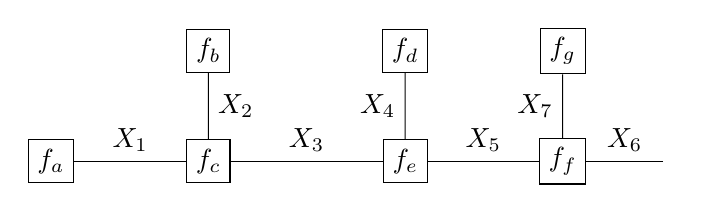
\begin{tikzpicture}[ scale=10, node distance=20mm, auto, >=latex' ] 


\node[factor] (fa) {$f_a$}; 
\node[factor,right of=fa] (fc) {$f_c$} edge[-] node[above] {$X_1$} (fa);
\node[factor,short,above of=fc] (fb) {$f_b$} edge[-] node[right] {$X_2$} (fc); 
\node[factor,long,right of=fc] (fe) {$f_e$} edge[-] node[above] {$X_3$} (fc); 
\node[factor,short,above of=fe] (fd) {$f_d$} edge[-] node[left] {$X_4$} (fe); 
\node[factor,right of=fe] (ff) {$f_f$} edge[-] node[above] {$X_5$} (fe);
\node[factor,short,above of=ff] (fg) {$f_g$} edge[-] node[left] {$X_7$} (ff); 
\node[terminal,short,right of=ff] (fh) {} edge[-] node[above] {$X_6$} (ff);

%\node[terminal] (fX1) { };
%
%\node[factor,right of=fA] (fB) {$f_B$} edge[-] node[below] {$X_3$} (fA); 
%\node[terminal,short,right of=fB] (fX5) {} edge[-] node[below] {$X_5$} (fB); 
%\node[terminal,short,below of=fA] (fX2) {} edge[-] node[left] {$X_2$} (fA); 
%\node[factor,short,below of=fB] (fC) {$f_C$} edge[-] node[left] {$X_4$} (fB); 



\end{tikzpicture}
\end{document}